% De Bruijn graph D(2,3) and an arborescence (generated by figs_c1ch09.py).
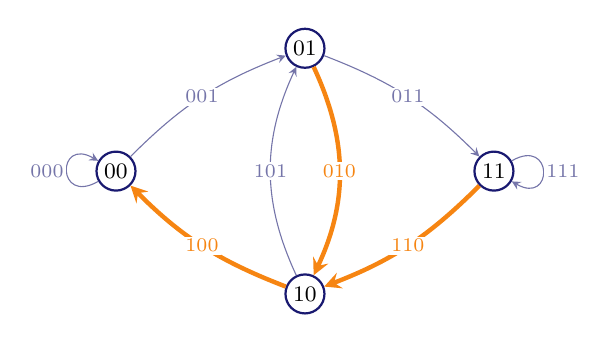
\begin{tikzpicture}[x=1.2cm,y=1.2cm,n/.style={circle,draw=MidnightBlue,thick,fill=white,inner sep=1.5pt,font=\footnotesize},a/.style={->,>=stealth,MidnightBlue!60},t/.style={->,>=stealth,BurntOrange,line width=1.6pt},l/.style={font=\scriptsize,fill=white,inner sep=1pt}]
\node[n] (00) at (0,0) {$00$};
\node[n] (01) at (2,1.3) {$01$};
\node[n] (10) at (2,-1.3) {$10$};
\node[n] (11) at (4,0) {$11$};
\draw[a] (00) to[out=210,in=150,looseness=6] node[l,left] {$000$} (00);
\draw[a] (00) to[bend left=12] node[l] {$001$} (01);
\draw[t] (01) to[bend left=25] node[l] {$010$} (10);
\draw[a] (01) to[bend left=12] node[l] {$011$} (11);
\draw[t] (10) to[bend left=12] node[l] {$100$} (00);
\draw[a] (10) to[bend left=25] node[l] {$101$} (01);
\draw[t] (11) to[bend left=12] node[l] {$110$} (10);
\draw[a] (11) to[out=30,in=-30,looseness=6] node[l,right] {$111$} (11);
\end{tikzpicture}
